% \subsection{Алгоритм для двунаправленных графов и языка Дика}

% \subsubsection{Мотивация (?)}

 % Например, рассмотреть неориентированные графы.

Для неориентированных графов отношение достижимости симметрично и на самом деле это отношение ``принадлежать одной компоненте связности''. Поддерживать добавление рёбер и проверку связности в неориентированном графе может СНМ. 

\subsection{Алгоритм, основанный на неориентированном транзитивном замыкании}

\textit{Я буду называть его Алгоритм НП}

В листинге~\ref{algo:NP} приведён псевдокод Алгоритма НП.

\begin{algorithm}[H]
    \floatname{algorithm}{Listing}
    \begin{algorithmic}[1]
    \caption{Алгоритм достижимости для РКА, основанный на неориентированном ТЗ}
    \label{algo:NP}
    \Function{UndirectedRSMReachability}{$\cool{R}$}
    % \Function{RSMReachability2}{$\cool{R}$}
        \State{$A \gets$ Empty adjacency matrix}
        \State{$Q \gets$ Empty Queue}
        \State{$D \gets$ DSU($|\bigcup\limits_{i=1}^k Q_i|$)}
        \For{$i \in 1..k$}
            \For{$u \xrightarrow{c} v \in \delta_i$}
                \State{$Q.Push(\q{u, v, i})$}
            \EndFor
        \EndFor
        \While{$Q$ is not Empty}
            \State{$\q{u, v, i} \gets Q.Pop()$}
            \If{$u \in En_i \wedge v \in En_i$}
                \Comment{Нашли новый путь}
                \State{$A \gets A \cup getEdges(i, u, v)$}
                \State{$Q.PushAll(getEdges(i, u, v))$}
                \State{$D.Union(u, v)$}
                \Comment{Добавляем новые рёбра}
            \EndIf
        \EndWhile
    \State \Return $A$
    \EndFunction
    \end{algorithmic}
\end{algorithm}

Для реализации алгоритма используются две вспомогательные структуры данных: очередь $Q$, хранящая рёбра, которые были добавлены в граф, но ещё не обработаны (как и в оригинальном алгоритме П2), и СНМ $D$, поддерживающая компоненты связности и поиск новых путей $\langle$стартовое состояние$\to$конечное состояние$\rangle$. 

Опишем подробно структуру используемого СНМ (в листинге~\ref{algo:DSU} приведён псевдокод.

\algblockdefx[Structure]{Structure}{EndStructure}
[1]{{\bf Structure} #1}
{}

\begin{algorithm}[H]
    \floatname{algorithm}{Listing}
    \begin{algorithmic}[1]
    \caption{Система Непересекающихся Множеств}
    \label{algo:DSU}
    \Structure{DisjointSets}
        \Function{DisjointSets}{$V$}
            \For{$v \in V$}
                \State{$P[v] \gets v$}
                \Comment{Предкок}
                \State{$R[v] \gets 0$}
                \Comment{Ранг}
            \EndFor
            \For{$v \in En(V)$}
                \State{$En[v] \gets \{v \}$}
                \Comment{Список стартовых вершин поддерева}
            \EndFor
            \For{$v \in Ex(V)$}
                \State{$Ex[v] \gets \{v \}$}
                \Comment{Список конечных вершин поддерева}
            \EndFor
        \EndFunction
        \Function{Find}{$v$}
            \If{$P[v] = v$}
                \Return $v$
            \EndIf
            \Return $P[v] = Find(P[v])$
            \Comment{Эвристика сжатие путей}
        \EndFunction
        \Function{Union}{$u, v$}
            \State{$u \gets Find(u)$}
            \State{$v \gets Find(v)$}
            \If{$u = v$}
                \Return
            \EndIf
            \If{$R[u] > R[v]$}
                \State{$Swap(u, v)$}
                \Comment{Ранговая эвристика}
            \EndIf
            \State{$Q.PushAll(\{ \q{en_u, ex_v}~|~en_u \in En[u], ex_v \in Ex[v] \})$}
            \State{$Q.PushAll(\{ \q{en_v, ex_u}~|~en_v \in En[v], ex_u \in Ex[u] \})$}
            \Comment{Добавление новых рёбер}
            \State{$En[v] \gets En[v] \cup En[u]$}
            \State{$Ex[v] \gets Ex[v] \cup Ex[u]$}
            \State{$R[v] \gets \max(R[v], R[u]+1)$}
            \State{$P[u] = v$}
            \Comment{Объединение компонент}
        \EndFunction
    \EndStructure
    \end{algorithmic}
\end{algorithm}

За основу взята стандартная реализация \cite{Hopcroft1973} на подвешенные деревья, использующая обе эвристики: сжатие путей и ранговую. 

% \TODO: \textit{Надо ли её расписывать?}

Дополнительно в корнях хранятся списки всех начальных и конечных состояний компоненты. При добавлении ребра в операции \textit{Join} перебираются все пары начальная/конечная вершина из двух компонент и соответствующие им рёбра добавляются в рабочую очередь $Q$. 

\TODO: (подумать) можно ли добавлять сразу много рёбер и сжимать их дфсом (как Борувка)?

\subsection{Время работы}

\begin{theorem}
На РКА из $n$ состояний и $m^{*}$ рёбрах в транзитивном замыкании, Алгоритм НП отработает за время $\O(n + m^{*} \alpha(m^{*} + n, n))$
\end{theorem}

\begin{proof}
~\\
\TODO: \textit{$m^{*}$ джойнов, а проходы по спискам не долгие, так как каждый раз генерируем новое ребро}
\end{proof}

\subsection{Корректность для неориентированных графов и некоторых классов грамматик}

\TODO: может, в мусорку этот subsection?

\subsection{Корректность для двунаправленных графов и языка Дика}

\textit{Напоминание, что для языка Дика контекстно-свободная достижимость $\to$ Дикова достижимость}

Для доказательства потребуется следующее вспомогательное утверждение

\begin{lemma}\label{lemma:bidir_equiv}
    Для вершин двунаправленных графов отношении Диковой достижимости является отношением эквивалентности.
    % For bidirected graphs the Dyck-reachability relation forms an equivalence, i.e., for all bidirected graphs $G$, for every pair of nodes $u$, $v$, we have that $v$ is Dyck-reachable from $u$ iff $u$ is Dyck-reachable from $v$.
\end{lemma}
\begin{proof}
~\\
\TODO: ну тут тупо

\end{proof}

\begin{note}    
    Для данного алгоритма будем использовать следующий вид грамматики для языка Дика:

    $S \to \eps~|~SS~|~(_1 S )_1~|~ \dots ~|~(_k S )_k$

    \begin{figure}[H]
        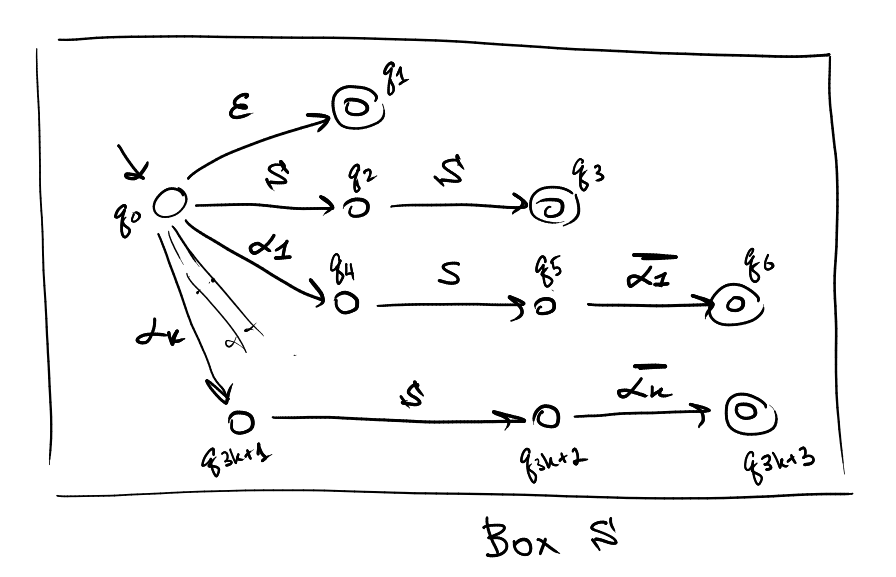
\includegraphics[width=0.75\linewidth]{img/dyck_box}
        \caption{РКА для языка Дика}
        \label{img:dyck_rsm}
    \end{figure}

    На рисунке~\ref{img:dyck_rsm} приведена РКА для данной грамматики. Заметим, что он содержит всего одну компоненту ($S$).

    \TODO: нарисовать красиво

\end{note}


\begin{theorem}
Решение для CFPQ, использующее Алгоритм НП, работает корректно на двунаправленных графах и языке Дика.
\end{theorem}
\begin{proof}

Достаточно доказать, что для любой пары состояний $u \in En_i, v \in Ex_i$ существование неориентированного пути эквивалентно существованию ориентированного.

% We only need to prove, that for every pair $u, v \in V(\mathcal{G})$ there is a path $(q_s, u) \rightsquigarrow (q_{f_i}, v)$ in ({\bf directed}) Kronecker product $G \otimes \mathcal{G}$ 
% iff 
% there is such path $(q_s, u) \rightsquigarrow (q_{f_j}, v)$ in an {\bf undirected} product (there $q_s$ is the initial state and $q_{f_i}, q_{f_j}$ are some final states of $G$ respectively).

$\Leftarrow$ (ориентированный $\SO$ неориентированный)

Очевидно, если есть ориентированный путь $u \path v$, то ровно если убрать ориентацию этот путь никуда не денется.

% Obviously (if $(q_{f}, v)$ is reachable from $(q_{s}, u)$ by directed edges, it is all the more reachable by undirected edges).

$\Rightarrow$ (неориентированный $\SO$ ориентированный)

% Для начала

At first, note that the Kronecker product $G \otimes \mathcal{G}$ forms some kind of a layered structure~--- $i$-th layer consists of vertices $(q_i, v)$, where $q_i$ is $i$-th RSM state. Because RSM is topologically sorted ({\color{red}{TODO}}), every edge $(q_i, u) \rightarrow (q_j, v)$ goes forward.

We will call path \textit{simple} if it visits every layer no more than once.

We prove the claim by induction on the $l$ (path length).

Clearly the result is true for $l \le 3$, because the only way to achive final vertex in $1, 2$ or $3$ edges is by a simple vertical path (which exists in the original graph too).

Otherwise (if $l \ge 4$), path is not simple. 

Consider the first flex point of the path, that is the vertex $(q_i, v)$ such that edges $(q_j, u) \rightarrow (q_i, v)$ and $(q_i, v) \rightarrow (q_k, w)$ are in the path and $j, k \le i$ (so, the path is convex at this point).

Looking at the grammar graph we can notice, that every state has indegree $\le 1$. So at the flex point there are actually two same-labeled edges (that is, $j = k$). 

There can be three different types of labels on those edges:

\begin{itemize}
    \item $\alpha_l$-label

        \textit{path: $(q_0, u) \rightarrow (q_i, v) \rightarrow (q_0, w) \rightarrow \dots \rightarrow (q_f, z)$.}

        Since $\alpha_l$-labeled edges could only be added on the initialization stage, 
        graph $\mathcal{G}$ contains edges $u \xrightarrow{\alpha_l} v$ and $w \xrightarrow{\alpha_l} v$. Notice, that cause $\mathcal{G}$ is bidirected, it also has to contain edges $v \xrightarrow{\overline{\alpha_l}} u$ and $v \xrightarrow{\overline{\alpha_l}} w$.

        Now we can notice, that $w$ is Dyck-reachable (by the path $\alpha_l \overline{\alpha_l}$) from $u$, so there is an $S$-labeled edge from $u$ to $w$. We can also conclude, that (by induction) there is a directed path from $(q_0, w)$ to $(q_f, z)$ (there $z$ is the end of the path and $q_f$ is some final state of $G$), so there is an $S$-labeled edge from $w$ to $z$. 

        Using this two observation we can construct a directed path from $u$ to $z$: $u \xrightarrow{S} w \xrightarrow{S} z$. 
    \item $S$-label

        \textit{path: $(q_0, a) \rightarrow \dots \rightarrow (q_j, u) \rightarrow (q_i, v) \rightarrow (q_j, w) \rightarrow \dots \rightarrow (q_f, z)$.}

        $\mathcal{G}$ contains $S$-labeled edges $u \xrightarrow{S} v$ and $w \xrightarrow{S} v$. Since $\mathcal{G}$ is bidirected, then by \ref{r1} $v \xrightarrow{S} u$ and $v \xrightarrow{S} w$. Combining $u \xrightarrow{S} v$ and $v \xrightarrow{S} w$ we get that $u \xrightarrow{S} w$. 

        No we want to sort of contract this edge, joining $u$ and $w$ (on the $j$-th level). Then we can get (by induction hypothesis) the directed path from $(q_0, a) \rightsquigarrow (q_f, z)$. If new path does not contain joined $uw$ vertex, then that's the answer. Otherwise we can split this vertex back, inserting between $u$ and $w$ the $S$-labeled path (that one, from $u \xrightarrow{S} w$ edge). We can do it, because the both of these paths form correctly matched parenthesis ({\color{red}{TODO}}: we can prove this using stack-based checking algorithm).

        \textit{Two other cases can be proved the same way, but I find it a little dishonest}

    \item $\overline{\alpha_l}$-label

        \textit{path: $(q_0, a) \rightarrow \dots \rightarrow (q_j, u) \rightarrow (q_f, v) \rightarrow (q_j, w) \rightarrow \dots \rightarrow (q_f, z)$.}

        Since $\alpha_l$-labeled edges could only be added on the initialization stage, 
        graph $\mathcal{G}$ contains edges $u \xrightarrow{\overline{\alpha_l}} v$ and $w \xrightarrow{\overline{\alpha_l}} v$. Notice, that cause $\mathcal{G}$ is bidirected, it also has to contain edges $v \xrightarrow{\alpha_l} u$ and $v \xrightarrow{\alpha_l} w$.

        By induction, we get that $a \xrightarrow{S} v$. Now we will construct a second part of the path: $(q_0, v) \xrightarrow{\alpha_l} (q_{j-1}, w) \xrightarrow{S} (q_j, w) \rightsquigarrow (q_f, z)$ ($q_{j-1}, w) \xrightarrow{S} (q_j, w)$ ~--- initial $S$-loop). By induction, we have directed simple version of this path, so $v \xrightarrow{S} z$. 

        Combining this two paths ($a \xrightarrow{S} v$ and $v \xrightarrow{S} z$) we get $a \xrightarrow{SS} z \Rightarrow a \xrightarrow{S} z$~--- desired path.
        
    \begin{figure}[H]
        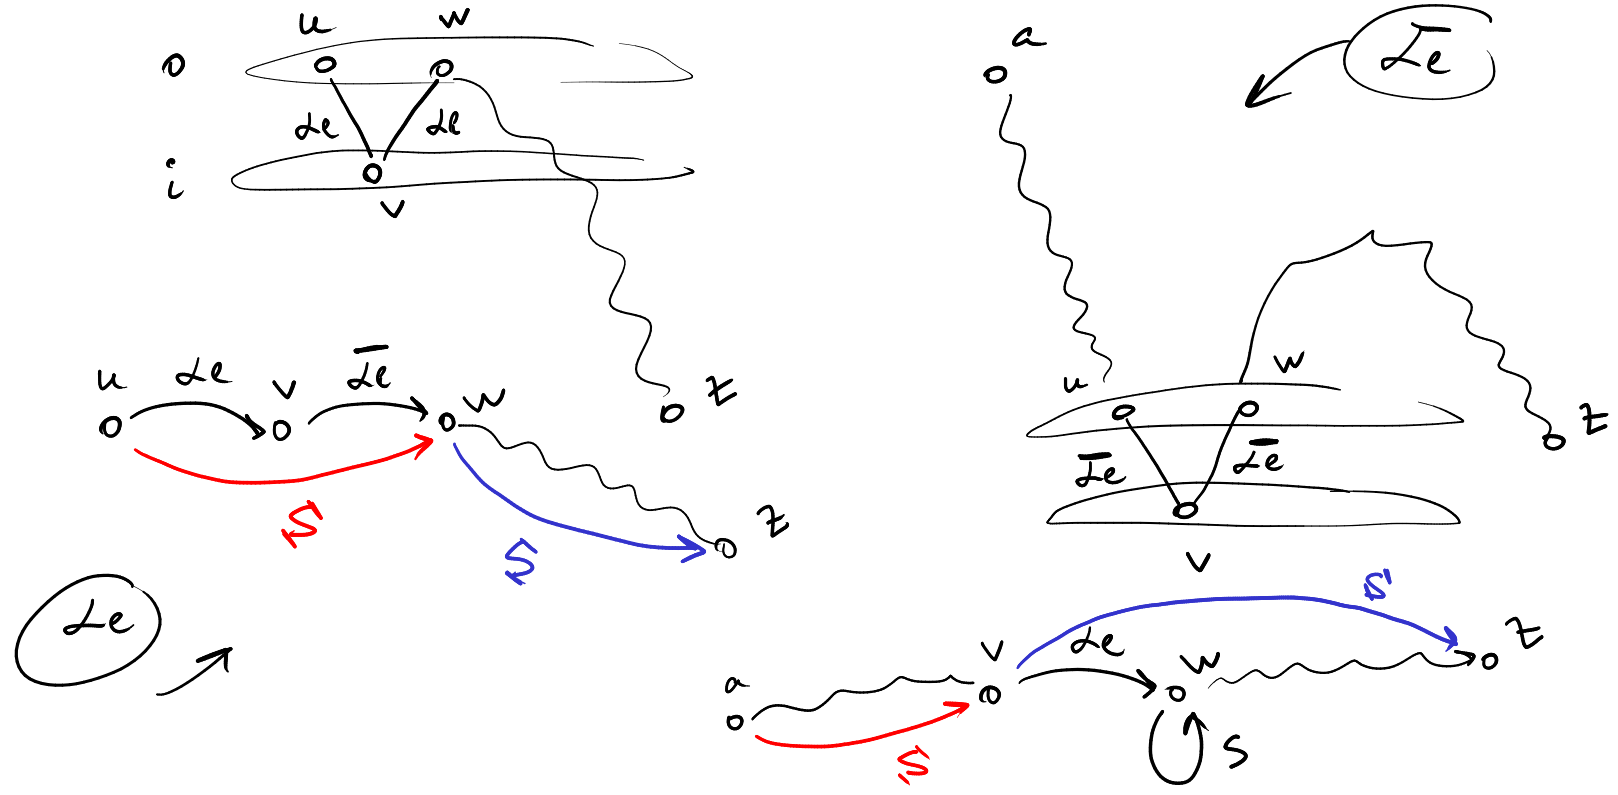
\includegraphics[width=\linewidth]{img/th_proof_img}
    \end{figure}
\end{itemize}

\end{proof}

\subsection{Выводы и результаты по главе}